\documentclass{article}

%% Packages 
\usepackage[english]{babel} % Language setting
\usepackage[a4paper,top=2cm,bottom=2cm,left=3cm,right=3cm,marginparwidth=1.75cm]{geometry} % Set page size and margins
\usepackage{amsmath}
\usepackage{graphicx}
\usepackage[colorlinks=true, allcolors=blue]{hyperref}
\usepackage{booktabs}
\usepackage{float} %\begin{table}[H] and table is where I want it
\usepackage{natbib} % it was just recommended by overleaf


%%%%%%%%%%%%%%%%%%%%%%%%%%%%%%%%%%%%%%%%%%%%%%%%%%%%%%%%%%%%%%%%%%%%%%%%%%%%%%%

%% Title
\title{Anonymization of data for open science in psychology: \\ 
       Part I — traditional anonymization
}
%% Authors
\author{Jiří Novák \and 
        Matthias Templ \and 
        Carolin Strobl
        }
        
%% Start of article %%%%%%%%%%%%%%%%%%%%%%%%%%%%%%%%%%%%%%%%%%%%%%%%%%%%%%%%%%%
%%%%%%%%%%%%%%%%%%%%%%%%%%%%%%%%%%%%%%%%%%%%%%%%%%%%%%%%%%%%%%%%%%%%%%%%%%%%%%%
\begin{document}
\maketitle

%% Abstract %%%%%%%%%%%%%%%%%%%%%%%%%%%%%%%%%%%%%%%%%%%%%%%%%%%%%%%%%%%%%%%%%%%
\begin{abstract}
\textcolor{red}{(Problem)} 
Psychology as a field has experienced a crisis caused by a lack of reproducibility. 
This has, on the one hand, led to distrust in the results, but on the other hand, it has enabled the development of open science practices. 
% One of the key parts of open science is open data, which must be well anonymized in order to be disseminated. 
A pivotal component of open science is the dissemination of well-anatomized open data, which facilitates transparency while protecting privacy.

Making more data openly available would make research more transparent and accessible. Unfortunately, many datasets cannot be shared even with other researchers for privacy reasons. 
%Nevertheless, researchers are increasingly more expected to share data with others for review, reanalysis, and reuse.
Despite these challenges, researchers are increasingly expected to make their data available for review, reanalysis, and reuse.

\textcolor{red}{(Methodology)} 
In this paper, we present good practices of statistical disclosure control for psychologists. 
The practices are divided into two separate parts: the first part consists of traditional approaches, and the second part focuses on the modern approach of using synthetic data.
The traditional approaches modify data so that it can be disseminated without revealing confidential information that may be associated with specific respondents. 

\textcolor{red}{(Conclusion)} \\ 
This paper seeks to provide practical insights into how statistical disclosure methods can effectively balance the need for data transparency and privacy in psychological research.
We include a detailed case study to demonstrate the practical application of these methods to protect sensitive data.

\end{abstract}

\keywords{
\textbf{Keywords:} 
open science, confidentiality, reproducibility, anonymization, privacy, statistical disclosure control, psychology
}

%%%%%%%%%%%%%%%%%%%%%%%%%%%%%%%%%%%%%%%%%%%%%%%%%%%%%%%%%%%%%%%%%%%%%%%%%%%%%%%
%% 1 - Introduction %%%%%%%%%%%%%%%%%%%%%%%%%%%%%%%%%%%%%%%%%%%%%%%%%%%%%%%%%%%
\section{Introduction}

%% Replication crisis %%%%%%%%%%%%%%%%%%%%%%%%%%%%%%%%%%%%%%%%%%%%%%%%%%%%%%%%%

%%%% Ideas
\textcolor{red}{— Discuss the Replication crisis (more lengthy on part I, part II paper citing part I paper)} \\
\textcolor{red}{— Discuss the importance of open science and data sharing. (more lengthy on part I, part II paper citing part I paper)} \\
\textcolor{red}{— State the aim of the paper, which is to explain statistical disclosure methods and showcase an anonymization or synthetization approach on a psychological dataset}

The replication and reproducibility crisis has received much attention in the last decade~\cite{2012_Yong}. The replication crisis is a phenomenon in science, particularly in psychology and medicine, in which many previously published scientific studies cannot be replicated or reproduced with consistent results. This means that when other researchers attempt to repeat the experiments using the original methodology, they fail to achieve the same outcomes. This issue raises concerns about the reliability and validity of scientific findings, leading to criticism of certain research practices, such as statistical errors, flawed experimental design, or the publication of only positive results.

In 2015, Open Science Collaboration~\cite{2015_OSC} of 271 authors examined the reproducibility of experiments in psychology. They selected about 100 studies from three psychology journals with the aim of achieving the same results as the original studies.  Only 36\% of original studies achieved significant results.
\textcolor{red}{Should I write more?}
\newline

%% Open science %%%%%%%%%%%%%%%%%%%%%%%%%%%%%%%%%%%%%%%%%%%%%%%%%%%%%%%%%%%%%%%
% In contemporary research, Open science practices are becoming increasingly important. Scientists process increasingly detailed data, which, however, in the field of psychology, are sensitive to the nature of the variables observed.
Open science practices are gaining importance in contemporary research, particularly in psychology, where researchers handle sensitive data. The sensitive nature of psychological variables often hinders data sharing, contributing to the reproducibility crisis in the field.
Therefore, data cannot be shared well among researchers, which is one reason for the crisis of scientific reproducibility. Data from publicly funded research should be more widely disseminated, at least among scientists. This would enable them to replicate studies, try new methods on the given data, or verify the results presented in the original article or study.
\newline

Open science is a movement that has been gaining strength and importance in recent years.
%The movement's goal is to make available the results of scientific research, arising on the basis of public finances, so that they are reusable and replicable, traceable and transparent, trustworthy, and more financially effective, enabling a better connection of science across the world.
The movement aims to make scientific research funded by public resources openly available to ensure it can be reused, replicated, traced, and trusted. This transparency also enhances the financial efficiency of research, fostering better global scientific collaboration.

It all started by Budapest Open Access Initiative~\cite{2012_OSI} in 2002, which was then supplemented by a set of rules in 2012~\cite{2012_OSI} and 2022~\cite{2022_OSI}.  This was followed by the Bethesda Statement on Open-Access Publishing~\cite{2003_Bethesda} in 2003 and the Berlin Declaration on Open Access to Knowledge in the Sciences and Humanities~\cite{2003_Max_Planck}.

Budapest Open Access Initiative (BOAI)~\cite{2002_OSI} defines the \textit{Open Access} (OA) as \textit{"free availability on the public internet, permitting any users to read, download, copy, distribute, print, search, or link to the full texts of these articles, crawl them for indexing, pass them as data to software, or use them for any other lawful purpose, without financial, legal, or technical barriers other than those inseparable from gaining access to the internet itself"}.

In recommendations from the 2012 BOAI~\cite{2012_OSI}, it was further specified that \textit{"The worldwide campaign for OA to research articles should work more closely with the worldwide campaigns for OA to books, theses and dissertations, research data, government data, educational resources, and source code."}. In 2022, new recommendations~\cite{2022_OSI} for the next 10 years were released. Strong emphasis was put on open infrastructure and its governance. The recommendation stated that OA texts, data, metadata, code, and other digital research outputs be hosted and published on open, community-controlled infrastructure. \textit{Open science} comprises open data, open metadata, open citations, open code, open protocols, open books, open theses and dissertations, open educational resources, open courseware, open digitization projects, open licenses, open standards, and open peer review.

From recent developments in recommendations for Open Science, it is necessary to mention the Commission Recommendation (EU) 2018/790 of 25 April 2018 on access to and preservation of scientific information~\cite{2018_EU_2018/790}, the European University Association (EUA) Open Science Agenda 2025~\cite{2022_EUA} and the UNESCO Recommendation on Open Science~\cite{2021_UNESCO}.

Recommendation 2018/790~\cite{2018_EU_2018/790} states that research data resulting from publicly funded research, including open access, should be findable, accessible, interoperable and re-usable, the so-called \textit{FAIR principles}, unless this is unfeasible or conflicts with the future use of the research findings. There should be a strong emphasis on the principle \textit{"As open as possible, as closed as necessary"}. 
The EUA~\cite{2022_EUA} established its Open Science strategy for 2025 with three main priority areas: Open Access to scholarly outputs, FAIR research data, and institutional approaches to research assessment. In the vision of the EUA for 2025, \textit{FAIR research data} is mentioned as the norm in producing and sharing scientific knowledge and \textit{Open Science} as an integral part of research assessment practices.

The UNESCO Recommendation~\cite{2021_UNESCO} defines \textit{Open Science} as \textit{"an
inclusive construct that combines various movements and practices aiming
to make multilingual scientific knowledge openly available, accessible and
reusable for everyone, to increase scientific collaborations and sharing of
information for the benefits of science and society, and to open the processes of scientific knowledge creation, evaluation and communication to societal actors beyond the traditional scientific community"}. In this recommendation, UNESCO promotes open access to scientific knowledge but equally emphasises the need for tools to pseudonymize and anonymize data so that as much data as possible can be shared appropriately.
\newline

%% Anonymization %%%%%%%%%%%%%%%%%%%%%%%%%%%%%%%%%%%%%%%%%%%%%%%%%%%%%%%%%%%%%%
Anonymization of personal information must be approached from the point of view of the field of statistical disclosure control (SDC). This research area is also known as statistical disclosure limitation or disclosure avoidance.
Hundepool~\cite{2012_Hundepool} describes SDC as a process that seeks to protect statistical data so that it can be released without divulging confidential information that can be linked to specific individuals or entities.

There are several major reasons for data anonymization, namely adhering to statistical principles, legal obligations, quality assurance, and ethical considerations. 

United Nations~\cite{2015_UN} list confidentiality of data as the sixth fundamental principle of Official Statistics. This principle states that the statistical records of individual persons, businesses, or events used to produce Official Statistics are strictly confidential and must be used only for statistical purposes. It is evident that this principle applies not only to Official Statistics but also to any other field processing sensitive information, which should secure the confidentiality of its records. The European Union defined this approach in its Code of European Statistics~\cite{2018_Eurostat} as the fifth principle — Statistical Confidentiality and Data Protection, which states that the privacy of data providers, the confidentiality of the information they provide, and its use only for statistical purposes and the security of the data are absolutely guaranteed.

Legislation imposes a legal obligation to protect individual business and personal data. Legal frameworks regulate what is allowed and what is not allowed regarding the publication of private information. In the member countries of the European Union, national statistical confidentiality is supported by EU legislation. The regulation of the European Parliament, better known by the abbreviation GDPR~\cite{2016_EU_2016/679}, is a pan-European legal framework for the protection of personal data, which protects the rights of citizens against unauthorized handling of their personal data.
In the context of the field of psychology, it is necessary to mention the United States legislation known as HIPAA~\cite{1996_HIPAA} - Health Insurance Portability and Accountability Act.
The HIPAA Privacy Rule establishes standards for the protection of individuals' medical records and other individually identifiable health information.

Quality assurance corresponds with the confidence of respondents in the preservation of the confidentiality of individual information. If they do not trust in the confidentiality of the data, they may not provide accurate information. United Nations~\cite{2007_UN} emphasizes that it is necessary to maintain respondents' trust if they are to continue to cooperate in data collection. If respondents perceive that the confidentiality of their data is not protected, they are less likely to provide accurate data.

Lastly, disclosing information that can be linked to specific individuals or entities is unethical. The Declaration on Professional Ethics~\cite{2010_ISI} sets a set of Ethical Principles for statisticians and a wide array of creators and users of statistical data and tools. 
Disclosing information that can be directly or indirectly linked to specific individuals or entities without their consent is considered unethical. Such actions may compromise privacy, lead to potential misuse of data, and violate principles of confidentiality. Ethical considerations require careful handling of sensitive information to prevent harm and uphold respect for personal and organizational boundaries. Appropriate steps must be implemented to ensure that data is released in a way that protects the confidentiality of individuals, preventing their identities from being disclosed or inferred.
\newline

%% Aim %%%%%%%%%%%%%%%%%%%%%%%%%%%%%%%%%%%%%%%%%%%%%%%%%%%%%%%%%%%%%%%%%%%%%%%%
This paper aims to explore and elucidate the various statistical disclosure control methods available for anonymizing data in the context of open science within psychology. 
It will focus on presenting a detailed examination of traditional anonymization methods and demonstrating their application to a psychological dataset. Through this analysis, the paper seeks to provide practical insights into how these methods can effectively balance the need for data transparency and privacy in psychological research.

%%%%%%%%%%%%%%%%%%%%%%%%%%%%%%%%%%%%%%%%%%%%%%%%%%%%%%%%%%%%%%%%%%%%%%%%%%%%%%%
%% 2 - Disclosure risk %%%%%%%%%%%%%%%%%%%%%%%%%%%%%%%%%%%%%%%%%%%%%%%%%%%%%%%%
\section{Disclosure risk}

%% 2.1 - General discussion on disclosure risk %%%%%%%%%%%%%%%%%%%%%%%%%%%%%%%%
\subsection{General discussion on disclosure risk}

\textcolor{red}{— Introduction and definitions of disclosure} \\
\textcolor{red}{— Somewhere we also need to explain what are direct, indirect identifiers, sensible variables, non-relevant variables for anonymization.}

Disclosure, also called re-identification, is the definition that is of the main interest when anonymising data.
Several definitions have been created over the years. 

In statistics, definitions are provided by SDC. Elliot~\cite{2009_Elliot}  describes disclosure as the inappropriate attribution of information to a data 
subject, whether through re-identification or by revealing sensitive attributes or memberships. Hundepool~\cite{2012_Hundepool} defines it as when a person or an organisation recognises or learns something that they did not already know about another person or organisation via released data. Templ~\cite{2014_Templ} similarly describes that it occurs when the intruder reveals previously unknown information about a respondent by using the released data.

In computer science, the definition can be found in the field of cybersecurity. The National Institute of Standards and Technology provides detailed guidelines and definitions for various cybersecurity concepts. Their glossary \cite{2023_NIST} defines unauthorized disclosure as \textit{“exposure of information to individuals who are not authorized to have access to it}”.  The most widespread is the concept of Differential privacy \cite{2006_Dwork} that, unlike traditional approaches that rely on identifying specific combinations of variables that could be re-identifiable, aims to ensure probabilistically that the information extracted from a database remains nearly unchanged after a new record is added. In other words, it adds carefully designed random noise to the data or the analysis process, making it extremely difficult to tell whether any one person’s data is in the dataset or not. 

From the legal point of view, the GDPR~\cite{2016_EU_2016/679}, do not define disclosure but use different term \textit{personal data breach} which means \textit{"a breach of security leading to the accidental or unlawful destruction, loss, alteration, unauthorised disclosure of, or access to, personal data transmitted, stored or otherwise processed"}. The GDPR encourages the use of pseudonymization as an effective means to enhance data security and reduce the risks associated with data processing, particularly in cases like data breaches or when processing sensitive data for research or statistical purposes. By pseudonymization is meant \textit{"the processing of personal data in such a manner that the personal data can no longer be attributed to a specific data subject without the use of additional information, provided that such additional information is kept separately and is subject to technical and organisational measures to ensure that the personal data are not attributed to an identified or identifiable natural person"}.
\newline

Methodology for safe data dissemination was coined in Official statistics by national statistical offices (NSO) and agencies a long time ago \cite{1977_Dalenius}. NSO developed these methods to release data  that enable users to gain insights and conduct original research while safeguarding the privacy of individuals in the dataset. 
These datasets are then released as Public Use File (PUF) or Scientific Use File (SUF). PUF and SUF are the most used terms in the European region; its definitions are codified in \cite{2009_EU_223/2009} and \cite{2015_EU_2015/759}. In the US, PUF is called Anonymised Microdata File, and SUF is called Licensed Microdata File. 

PUF is accessible to the general public, and for this reason, the highest level of security against the disclosure of respondents' personal data is required. The data contained in the file for public use must be anonymized in such a way that it does not allow, either directly or indirectly, to identify statistical units, taking into account all reasonable means, the use of which can reasonably be expected by a third party. 

SUF contain data that only approved researchers can access. A contract is usually signed at the same time as a guarantee of confidentiality. This type of data needs a lower level of security than PUF, but respondents' personal information is still protected from disclosure. Data contained in a file with confidential data for scientific purposes must be anonymized in such a way that allows only indirect identification of statistical units.

By direct identification \cite{2009_EU_223/2009} is meant \textit{the identification of a statistical unit from its name or address, or from a publicly accessible identification number} and indirect identification \cite{2009_EU_223/2009} is defied as  \textit{the identification of a statistical unit by any other means than by way of direct identification}.
\newline

Depending on the type of variable identification, Hundepool \cite{2012_Hundepool} categorized them into four categories: Identifiers, Quasi-identifiers or key variables, Confidential outcome variables, and Non-confidential outcome variables. These categories are not disjoint.

Identifiers are variables that directly and uniquely identify an individual respondent. Examples include details such as participant ID numbers, full names used in therapeutic settings, or unique patient numbers in mental health services. Since SDC aims to prevent the identification of individuals, these identifiers are typically removed or encrypted before processing the data.

Quasi-identifiers or key variables are variables that, in combination with other external data, can be used to identify individuals within the dataset. Unlike identifiers, these cannot be easily removed because almost any variable could act as a quasi-identifier based on the available external information. Examples from psychology include age, gender, and location of a participant in an anxiety study (as a specific combination might be identifiable); education level and job title in a stress study (these, combined with geographic information, may allow re-identification); or a specific school and role in a burnout study involving teachers (such as identifying the principal of a certain school).

Confidential outcome variables include sensitive information about respondents, which could pose risks if disclosed. Examples from psychology are diagnoses of mental health conditions (e.g., depression, PTSD), history of substance use or addiction, and sensitive scores from psychometric assessments like the Beck Depression Inventory.

Non-confidential outcome variables do not directly contain sensitive information but still need to be considered during data protection because they can form part of a quasi-identifier. Examples include general information such as participation in a type of therapeutic intervention (e.g., cognitive behavioral therapy, without specifying the underlying reason), number of siblings or children in a family dynamics study, and exercise habits in research on general well-being. Even though they seem non-sensitive, a combination like “Job title” and “Town” could potentially identify a specific individual, such as a doctor in a small village.
\newline

Templ \cite{2017_Templ} also provides an additional classification for more complex data sets, where he described in detail Linked Variables, Sampling weight and Hierarchies, Clusters, and Strata.

Linked variables are variables in the dataset that are related to key variables and should be treated similarly when anonymizing data. For example, if a key variable (e.g. income) is suppressed for privacy reasons, a linked variable (e.g. tax payment) should also be suppressed. This ensures consistency in the anonymization process and prevents scenarios where suppressed data could still be inferred indirectly through its related variables. Linked variables are particularly important when applying methods like suppression, where related values must be considered to maintain data protection. 
An example from Psychology is a situation when a participant's occupation is suppressed as a key variable. Their job title (if available as a separate variable) should also be treated in the same way to prevent indirect identification.
Suppose a study on mental health includes detailed work environment variables that are connected to occupation. If the occupation is masked for anonymity, details on the work environment must be consistently suppressed.

Sampling weights are variables used to adjust data for unequal selection probabilities, often present in survey datasets. These weights are crucial in reflecting the actual population but may also carry confidential information. The presence of sampling weights can influence disclosure risk, as they provide insight into the population or specific subgroups. Proper care is needed when anonymizing microdata that includes sampling weights to ensure that these weights do not enable re-identification or reveal sensitive information indirectly.
An example from Psychology could be that in a survey about childhood stress levels, sampling weights are applied to account for the overrepresentation of children from specific regions. Care must be taken to ensure that these weights do not allow the identification of participants from smaller, uniquely sampled subgroups.

Data may have hierarchical structures, such as clusters or strata, which are typical in survey sampling designs. Hierarchies may reflect relationships within data, like households or organizational levels, which need special handling in anonymization. Clusters refer to groups where individuals share some common characteristics (e.g., classrooms or neighborhoods). Strata are used in sampling to ensure the representation of different population segments. The presence of hierarchies, clusters, and strata increases the disclosure risk, as individuals within the same cluster tend to be similar. When managing microdata, it is essential to anonymize while maintaining these structures without revealing information that could lead to identification within these groups.
Example Psychology is that in a psychological study of family dynamics, the data is collected from multiple families, with each family considered a cluster. To protect individuals’ privacy, anonymization must consider the relationships between family members while also ensuring that identifying characteristics, such as family size, do not inadvertently expose identities.
Another example could be school-level data, where children in different grades are grouped. Protecting one individual’s data requires ensuring that identifying information at the class or school level does not expose other students.

%% 2.1 - Types of Disclosure %%%%%%%%%%%%%%%%%%%%%%%%%%%%%%%%%%%%%%%%%%%%%%%%%%
\subsection{Types of Disclosure}

%Disclosure risks that may occur are identity disclosure, attribute disclosure, defined by~\cite{1989_Duncan}, and inferential disclosure, defined by~\cite{1977_Dalenius}.

In statistics, three basic types of disclosure \cite{1993_Lambert}~\cite{1989_Duncan}~\cite{1977_Dalenius} are commonly recognized: identity disclosure, attribute disclosure, and inferential disclosure. These types are well discussed in Hundepool \cite{2012_Hundepool}, Templ \cite{2017_Templ}, and Garfinkel \cite{2023_NIST}. From a computer science perspective, Rigaki \cite{2024_Rigaki} identified four categories: membership inference, reconstruction, property inference, and model extraction. For psychology, we recommend using the following statistical definitions of disclosure.

\begin{figure}[H]
    \centering
    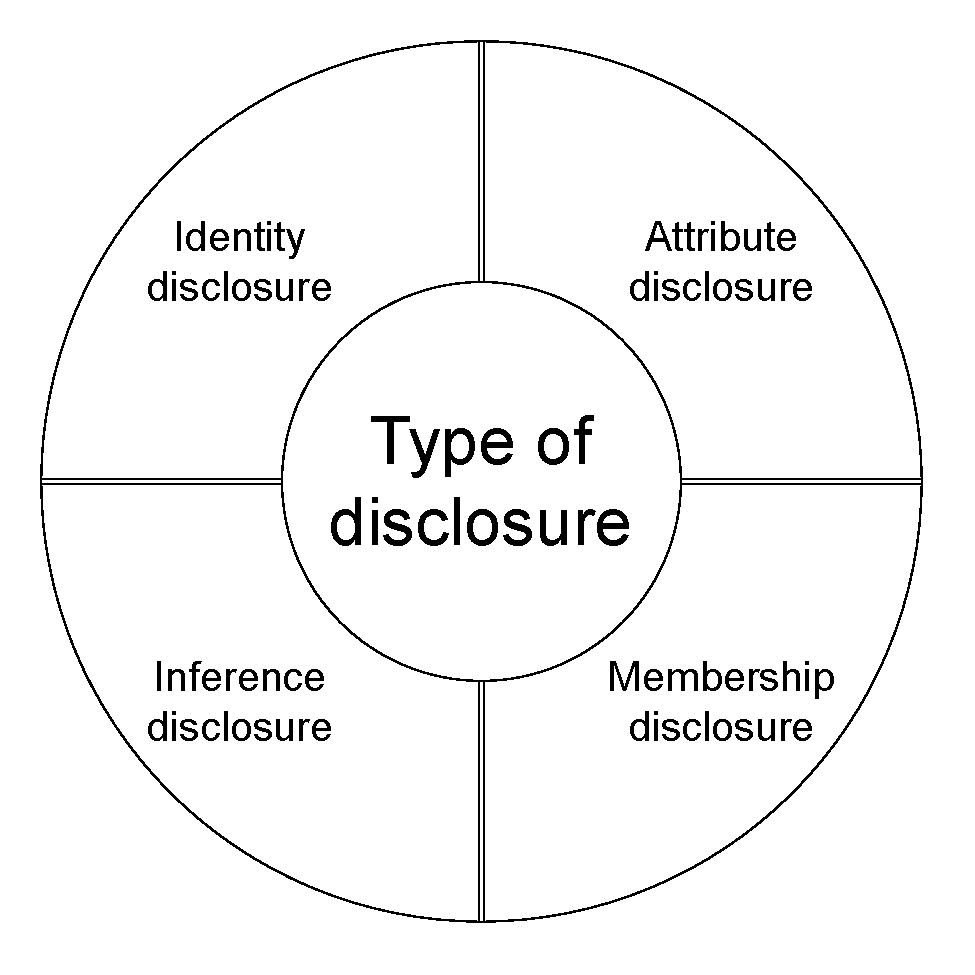
\includegraphics[width=0.5\linewidth]{Drawio/Type_of_disclosure.drawio.pdf}
    \caption{Types of disclosure}
    \label{fig:Types_of_disclosure}
\end{figure}

% Identity disclosure
\paragraph{Identity disclosure:} 
Occurs when an individual’s identity is revealed, thereby allowing someone to link that individual to specific records or data points in a dataset. Identity disclosure occurs when the information provided is unique or detailed enough to enable re-identification, even if direct identifiers (e.g. name, address) have been removed. This form of disclosure poses a significant privacy risk because once an individual is re-identified, all associated data points are also disclosed.

In psychological and behavioral research, identity disclosure is a critical concern, as participants may provide highly sensitive personal information, such as emotional well-being, interpersonal relationships, or medical history. Identity disclosure may occur if someone can cross-reference quasi-identifiers (such as age, zip code, occupation) with other external data sources.

Example:
Suppose a participant in a psychological study discloses their gender, age, occupation, and city of residence. If that combination is unique enough, especially in a small community, it may be possible for someone with access to auxiliary information (such as a local registry) to determine the individual’s identity, linking them to the study’s sensitive information.

%% Attribute Disclosure
%\paragraph{Attribute Disclosure:} 
%Attribute disclosure \cite{2012_Hundepool} happens when certain traits or characteristics of a participant can be deduced without knowing their identity directly. This type of information leakage is particularly concerning when publishing data in tables, as empty cells in the table can unintentionally reveal information. For example, if a group of participants is represented in a table and an empty cell appears, an observer may deduce that no participant in that group has the combination of attributes represented by the empty cell. This form of disclosure can compromise privacy even without directly identifying the individuals.

\paragraph{Attribute Disclosure:} 
\color{blue}
Occurs when specific information or attributes about an individual are revealed without necessarily identifying the person themselves. Even if the individual’s identity remains anonymous, sensitive characteristics or behaviors linked to them may be disclosed, leading to potential privacy risks. In other words, attribute disclosure doesn’t rely on knowing who a person is but rather on revealing what is true about them. This can have harmful consequences, especially when the disclosed attributes are sensitive, stigmatized, or could lead to discrimination.

In psychological and psychometric data, this can be particularly problematic because participants often provide highly personal and sensitive information—such as mental health status, personality traits, or risky behaviors—that they would not want disclosed, even if their names are not attached to the data. Attribute disclosure can happen if the characteristics of a person are unique enough or if those attributes can be inferred through combining seemingly innocuous pieces of information (like age, location, or gender) with responses on psychological scales or ratings.

Example: 
Suppose a research participant has filled out a questionnaire that includes both socio-demographic information and responses to a sensitive mental health scale, such as one measuring depression or anxiety. Someone might not know the exact identity of the participant but could still infer that someone within a particular group (e.g., women over 50 with a specific level of education) has a high score on the depression scale, which could lead to conclusions about members of that group.

Why Attribute Disclosure is harmful:
\cite{2022_Wairimu} and Kilovaty \cite{2021_Kilovaty} highlight how sensitive information, such as diagnoses or treatments, may be revealed in ways that lead to embarrassment, stigmatization, or discrimination. This exposure can come from family, friends, the wider public, or organizations that may misuse this information, affecting an individual’s well-being. The authors emphasize that attribute disclosure can still occur if identifiable details like demographics are masked but correlate with sensitive information in clinical or psychometric studies.
For instance, consider a situation where a patient's demographic information is generalized, but their responses or scores on a study about paranoid schizophrenia could still expose their diagnosis. In this case, the mental health data, although anonymized, might be used to infer sensitive personal information about the individual, leading to potential harm. In psychometrics, this is particularly problematic, as attributes being disclosed often pertain to deeply personal issues—such as mental health, personality, or behaviors—where even indirect exposure can result in stigma, discrimination, or embarrassment for both individuals and groups.
\color{black}

%% Inferential disclosure
\paragraph{Inferential disclosure:}
Occurs when sensitive information about an individual can be inferred, even if that individual’s identity is not explicitly revealed. Inferential disclosure can happen when someone makes educated guesses about an individual based on available data patterns or statistical models. This is particularly concerning when the inferred information is of a confidential or sensitive nature, as it can lead to privacy violations without directly identifying someone.
In psychological studies, inferential disclosure can happen when responses to certain survey questions or psychometric measures can be used to derive or predict private information. Even without directly linking data to an individual, conclusions can be made that may reveal details about a participant’s mental state or experiences.

In psychological studies, inferential disclosure can happen when responses to certain survey questions or psychometric measures can be used to derive or predict private information. Even without directly linking data to an individual, conclusions can be made that may reveal details about a participant’s mental state or experiences.

Example:
Imagine a dataset from a psychological study that contains participants' scores on a stress management scale along with their occupation. Suppose the data shows that teachers tend to have lower scores on stress management, indicating higher stress levels. If someone knows that a specific individual is a teacher and participated in the study, they could infer that this individual likely has difficulty managing stress, even without knowing which exact record belongs to them. This inference could lead to negative judgments or assumptions about that person.

%% Inferential disclosure
\paragraph{Membership disclosure:}
Occurs when it is revealed whether an individual is part of a specific dataset or participated in a particular study. Membership disclosure does not necessarily reveal sensitive information about an individual but indicates that they are associated with a particular group. This kind of disclosure can still pose privacy risks, especially if the dataset involves stigmatized or sensitive topics. Knowing that someone is part of a dataset related to mental health issues, for example, could lead to unwanted judgments or discrimination

In psychological research, membership disclosure can be particularly problematic when the dataset pertains to sensitive conditions or behaviors, such as mental health diagnoses, substance use, or intimate personal experiences. Even if specific attributes or identifiers are not disclosed, the mere association with such a dataset could impact an individual’s privacy and lead to negative consequences.

Imagine a study involving individuals with a history of addiction. Even if no personal details are shared, revealing that someone participated in the study implies their association with addiction. This disclosure could have social or professional repercussions for the individual, especially if others can infer their membership from auxiliary information, such as demographic or geographic clues available from other sources.

%% 2.1 - Attacker scenarios %%%%%%%%%%%%%%%%%%%%%%%%%%%%%%%%%%%%%%%%%%%%%%%%%%%
\subsection{Attacker scenarios}

These scenarios describe the different methods adversaries might use to compromise individuals' privacy. The scenarios depend on the intruder's intentions, prior knowledge, and the available data.
Depending on the intention of the intruders, their type of a priori knowledge and the data available.

%% Nosy neighbor
\paragraph{Nosy neighbor:}
\color{blue} % Suggestion from Matthias

In this type of attack, the attacker has existing knowledge of one or more individuals in the dataset. This knowledge may include  private knowledge, such as participation in a study or specific responses. By comparing this background information to anonymized data, the attacker can isolate the individual's record and infer sensitive attributes, such as mental health status, survey responses, or psychometric scores.

Example:

Imagine an attacker knows that a 42-year-old female manager from a specific region participated in a psychological study on workplace stress. While the data set is anonymized, it contains enough socio-demographic information, such as age, occupation, and region, to make the participant’s record unique. The attacker cross-references this knowledge and identifies the specific individual in the data set. Once identified, the attacker could then infer sensitive responses—such as scores on a stress or mental health scale—that the individual had shared under the assumption of anonymity.
Also participants that complete psychometric assessments such as a well-being scale (e.g., the satisfaction with life scale or a loneliness measure) alongside data about their social network can be disclosed by friendship links, which might carry significant information to disclose sensitive information \citep{Zheleva09}.

Risk: The risk of a background knowledge attack increases when individuals have unique or rare combinations of attributes within the dataset, making them more identifiable. Attributes like age, gender, occupation, education level, and location -- while seemingly non-identifiable on their own -- can become identifiable when combined in specific ways. There is always a high risk that a ‘nosy neighbor’ who knows very specific details about a person (e.g., their movements when studying how depressive symptoms and anxiety levels correlate with daily mobility patterns, available as GPS data) could use this information to link the individual to publicly released open-access data.

\color{black}  % End of Suggestion

%% Linkage attacks
\paragraph{Linkage attacks:}
A linkage attack \cite{2012_Hundepool} occurs when an adversary attempts to re-identify individuals in a dataset by linking quasi-identifiers (e.g., age, gender, location) with other publicly available data. This attack exploits the fact that certain combinations of quasi-identifiers may uniquely identify an individual.

Example: In a psychological dataset, information such as "female, aged 45, resident of a small town" might be linked with voter registration data or social media profiles to identify the individual and learn their sensitive survey responses.

%% Outlier attack
\paragraph{Outlier attack:}


%% 
\paragraph{Differential attack:}
A differential attack \cite{2008_Dwork} occurs when an adversary compares two versions of a dataset, one of which contains data on a specific individual and the other does not. By observing the differences between the datasets, the attacker can infer information about that individual. Differential privacy is designed to protect against this kind of attack by adding noise to the data.

Example: If an individual participated in a psychological survey, an attacker could compare a dataset with and without that individual's data to learn information about the changes in summary statistics or other aggregated results, revealing sensitive information about the individual.

%% 
\paragraph{Homogeneity attack:}

%% 
\paragraph{Inference attack:}
X
\newline

\begin{table}[H]
    \centering
    \begin{tabular}{lcc}
        Scenario & X & X \\
        Nosy neighbor & X & X \\
        Linkage attacks & X & X \\
        Differential attack & X & X \\
        Homogeneity attack & X & X \\
        Inference attack & X & X \\
    \end{tabular}
    \caption{Attacker scenarios}
    \label{tab:tab1}
\end{table}


\begin{figure}[H]
    \centering
    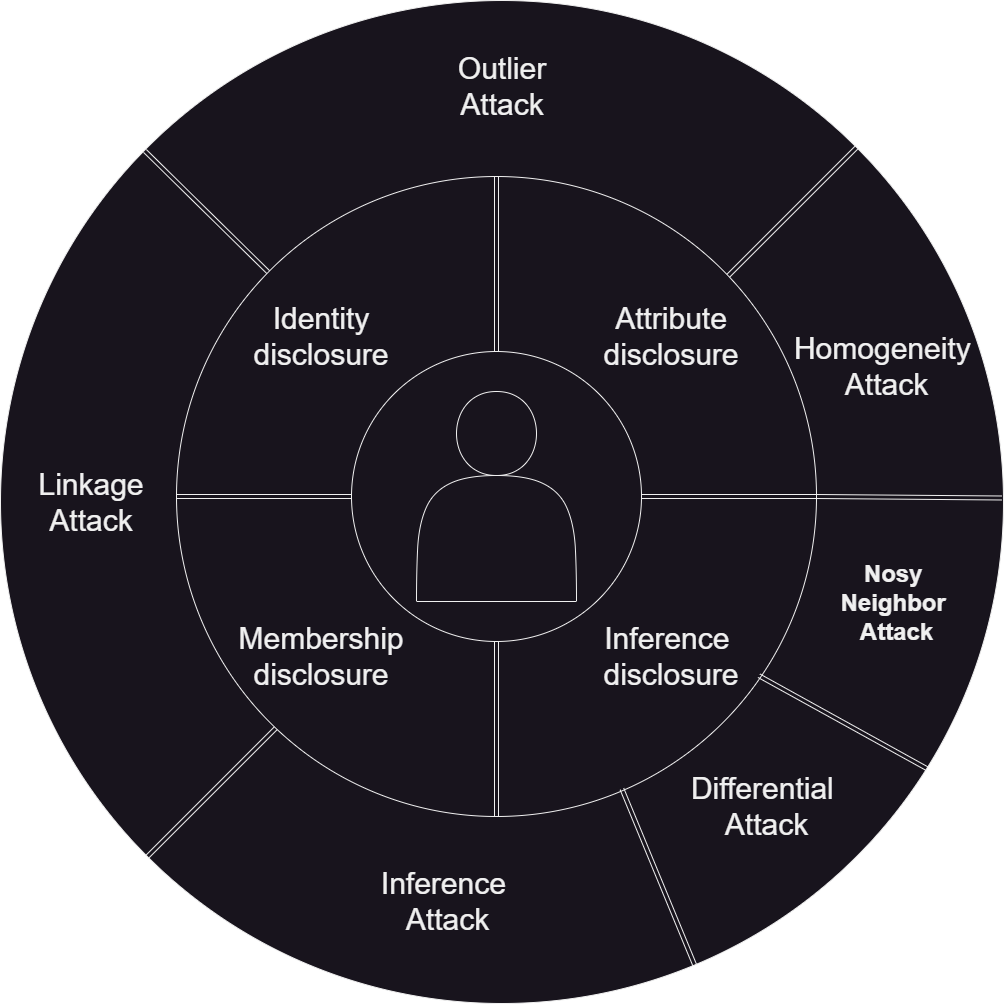
\includegraphics[width=0.5\linewidth]{Drawio/Type_of_disclosure_attacks.pdf}
    \caption{Disclosure attacks}
    \label{fig:Disclosure_attacks}
\end{figure}

%% 2.3 - Kind of data %%%%%%%%%%%%%%%%%%%%%%%%%%%%%%%%%%%%%%%%%%%%%%%%%%%%%%%%%
\subsection{Kind of data}

\paragraph{Survey and questionnaire data}
-type
- risk
- data structure
- anonymization needs

\paragraph{Qualitative data:}

\paragraph{Psychometrics score:}

\paragraph{Longitudinal data:}

\paragraph{Biometrics and psychological data:}

\paragraph{Behavioural data (eye tracking, ...):}

\paragraph{Genetic data:}

\paragraph{Social network data:}
X

\begin{table}[H]
    \centering
    \begin{tabular}{lcc}
        Data & X & X \\
        Survey and questionnaire data & X & X \\
        Qualitative data & X & X \\
        Psychometrics score & X & X \\
        Longitudinal data & X & X \\
        Biometrics and psychological data & X & X \\
        Behavioural data & X & X \\
        Genetic data & X & X \\
        Social network data & X & X \\
    \end{tabular}
    \caption{Kinds of data}
    \label{tab:tab2}
\end{table}

\subsection{Data precularies}

\color{blue} 
Suggestion from Matthias
\color{black}

\begin{table}[H]
\begin{small}

    \centering
    \begin{tabular}{p{2cm}|p{2cm}|p{2cm}|p{3cm}|p{5cm}|}
    \toprule
       kind of data  & structure  & sensitivness & risk & anonymization \\
       \midrule
       Psychometric test scores   & highly granular, often highly correlated & can be high & sensitive attribute disclosure (e.g., mental health diagnosis, personality traits) can occur if linked with other data or demographic profiles. & difficult to generalize or group psychometric item responses without losing significant information about the underlying construct being measured. Often enough to anonymize indirect identifiers, when potential attackers know little about the measurement of the items. \\
       \midrule
       &&&& \\
       \bottomrule
    \end{tabular}
    \caption{Common data structures in psychology and psychometrics and their relationship to disclosure risk and anonymization.}
    \label{tab:my_label}

\end{small}
\end{table}



%% 2.4 - Evaluating disclosure risk %%%%%%%%%%%%%%%%%%%%%%%%%%%%%%%%%%%%%%%%%%%
\subsection{Evaluating disclosure risk}

Similar to the definition of disclosure, different approaches in statistics and informatics are used to evaluate the risk of disclosure. The most used approach in statistics is k-anonymity \cite{2002_Sweeney}, and in computer science, it is differential privacy \cite{2006_Dwork}. Both are mathematically rigorous methods aimed at enabling the controlled use of confidential data while minimizing privacy risks to individuals. Although both are formal privacy models, k-anonymity focuses on ensuring privacy through the content of the released data, whereas differential privacy limits the information that can be inferred about the confidential data from the released dataset.

When using these approaches, it is necessary to take into account the trade-off between the information loss of the published data and the usefulness and accuracy of the given dataset.
By accuracy \cite{2008_OECD}, it is meant \textit{“closeness of computations or estimates to the exact or true values that the statistics were intended to measure”}
By usefulness or utility \cite{2023_NIST}, we refer to the overall value that users can obtain from the data.
Generally, data accuracy decreases as more intensive anonymization techniques are applied. 
However, increased privacy protections do not always lead to reduced data utility for specific purposes. 
Balancing the competing demands of data accuracy, utility, and privacy remains one of the key challenges of data anonymization, necessitating careful consideration of each dataset's specific goals and context.

\paragraph{Uniqueness}

\paragraph{k-anonymity:}

\color{blue}
$k$-Anonymity is a privacy protection mechanism that ensures each individual in a dataset cannot be distinguished from at least $k$  other individuals based on certain identifying attributes. In the context of psychology and psychometry, $k$-anonymity can be used to protect sensitive data (such as mental health scores, socio-demographic characteristics, or mobility patterns) by making sure that participants’ data entries are indistinguishable from those of at least $k$  others based on specific quasi-identifiers (e.g., age, gender, occupation).  $k$-anonymity is evaluated on the indirect-identifiers. For example, in \citep{schoenbrodt21} the authors measured (and anonymized the data using \cite{2024_Sdcmicro} to achieve) $5$-anonymity for a data base responses to 54 classic and new picture stimuli that have
been used in picture story exercise to measure coding motive imagery in a psychometrics study regarding their key variables age and gender.
\color{black}

\paragraph{l-diversity}

\paragraph{t-closeness}

\paragraph{risk scores}

\paragraph{individual risk when survey samples}



\subsection{xxxxxxxxxxxxxxxxxxxxxxxvxxxx}

Statistical Disclosure Control (SDC), as defined by~\cite{2012_Hundepool}, seeks to protect statistical data in a way they can be released without revealing confidential information that can be linked to specific individuals. The goal of SDC methods is to find an optimal solution for both the risk of disclosure and the utility of protected published data.


\newline
















The first step of anonymization is evaluating risks that threaten the data. This is approached by creating disclosure scenarios~\cite{2012_Hundepool} tailored to the data that will be disseminated. 


%%%%%%%%%%%%%%%%%%%%%%%%%%%%%%%%%%%%%%%%%%%%%%%%%%%%%%%%%%%%%%%%%%%%%%%%%%%%%%%
%% Disclosure attackss %%%%%%%%%%%%%%%%%%%%%%%%%%%%%%%%%%%%%%%%%%%%%%%%%%%%%%%%
\subsection{Disclosure scenario}

\textcolor{red}{— Review existing literature on statistical disclosure control methods (with focus on applications in  psychology/psychometrics)} \\
\textcolor{red}{— Discuss specific challenges and considerations or anonymizing of data in psychology/psychometrics.} \\
\textcolor{red}{— Discuss the possibilities on utility measurement} \\
\textcolor{red}{— Discuss the disclosure scenarios (basically for anonymization: identity and attribute disclosure; for synthetic data: membership and inferential disclosure)} \\


From these scenarios, the types of data disclosures emerge.

At the beginning of the SDC process, data must be cleaned of direct identifiers such as name, social security number or similar ID, address, and e-mail. This is called de-identification~\cite{2001_Duncan} or pseudo-anonymization. This alone does not prevent de-identification and revealing new information to the intruder.





\paragraph{Identity disclosure:} is the association or linking of the specific respondent to a record. Preventing this is of great importance. 










Dissemination of findings from psychological science is discussed by Purtle \cite{2020_Purtle}, they advocate for a structured, evidence-based approach to effectively communicating psychological research by conducting audience research, segmenting target groups, and testing dissemination strategies, with attention to personalization and privacy concerns. However, the article does not provide detailed guidance on how to ensure privacy during the dissemination process.

Couper \cite{2008_Couper} examined how perceptions of privacy, confidentiality, or risk of data disclosure affect individuals' willingness to participate in surveys. The findings show that while objective disclosure risk does not significantly reduce survey participation, perceptions of risk and topic sensitivity substantially lower the willingness to participate. Respondents are more likely to decline participation in surveys on sensitive topics, driven by concerns about privacy and potential harm, rather than the actual probability of data disclosure.

Last but not least, Kilovaty \cite{2021_Kilovaty} describes that the disclosure of sensitive data can lead to profound emotional and psychological consequences, including heightened anxiety, depression, post-traumatic stress disorder, and a range of other mental health challenges that can severely impact the well-being of those affected.

Wairimu \cite{2022_Wairimu} collected real-world examples of privacy breaches in healthcare.
% 1 
These include a case where a nurse in Florida disclosed a woman’s medical records, causing fear and embarrassment. The nurse’s actions, which involved sharing sensitive information with unauthorized individuals, highlighted the dangers of improper access to personal medical data\footnote{https://www.tampabay.com/archive/2013/06/29/records-breach-lets-out-secret/}.
% 2 
In the case of Hinchy v.Walgreen Co., a patient’s prescription history was shared with her ex-boyfriend, leading to emotional distress. The court found Walgreens liable for both HIPAA violations and negligence, resulting in a \$ 1.44 million judgment against the company\footnote{https://www.bswllp.com/the-intersection-of-hipaa-and-negligence-pharmacists-violation-cost-walgreens-144-million}. 
% 3 
Hackers leaked the medical data of high-profile athletes from the World Anti-Doping Agency, exposing sensitive medical information about the athletes and potentially causing distress for the athletes involved\footnote{https://www.bbc.com/news/world-37369705}. 
% 4
One patient’s HIV status was publicly accessible for months, which occurred when her medical information was shared inappropriately. This breach not only caused emotional harm but also led to feelings of fear, stigma, and a profound loss of trust in the healthcare system, leading to significant emotional harm\footnote{https://www.npr.org/sections/health-shots/2015/12/10/459091273/small-violations-of-medical-privacy-can-hurt-patients-and-corrode-trust}. 
% 5 
One victim of medical identity theft incurred nearly \$20,000 in fraudulent bills, causing financial strain and distress. It was caused by hackers stealing medical records and selling them on the dark web. These data often include sensitive personal information like Social Security numbers, birth dates, and medical histories\footnote{https://www.cbsnews.com/news/hackers-steal-medical-records-sell-them-on-dark-web/}. 
% 6
%A woman’s medical records were unlawfully accessed by her ex-partner, leading to anxiety and stress\footnote{https://www.hayesconnor.co.uk/news-resources/case-study/woman-has-her-medical-records-unlawfully-accessed-by-her-ex/}. 
% 7
An NHS staff member unlawfully accessed and shared a relative's confidential medical records with other family members, which resulted in psychological harm and medication use. 
The case emphasizes the serious consequences of mishandling personal medical data, even within families\footnote{https://www.hayesconnor.co.uk/news-resources/case-study/nhs-family-member-shared-confidential-medical-information/}. 
% 8
% Another case involved a patient’s HIV status remaining publicly accessible for months, causing emotional distress and embarrassment.
% 9
In Finland, psychotherapy patients were subjected to blackmail after a data breach. The hackers obtained highly confidential patient records, including details of therapy sessions, and then attempted to blackmail both the patients and the psychotherapy clinic. Victims received ransom demands threatening to publicly release their personal mental health information if payments were not made. The breach caused widespread distress among patients and raised concerns about the security of sensitive medical data in the healthcare sector.\footnote{https://www.theguardian.com/world/2020/oct/26/tens-of-thousands-psychotherapy-records-hacked-in-finland}. 
% 10
%A doctor in California shared a patient’s full medical records with an investigator for personal revenge. \footnote{https://www.nzherald.co.nz/nz/breach-of-doctors-privacy-by-colleagues-condemned-by-medical-authorities-unions/US35AYFBYZRX6DZKWUWKRRE6AE/}. 
% 11
In a UK case, women were stalked after the unauthorized access occurred following a data breach at University Hospital Crosshouse in Scotland, where the woman's details were improperly shared\footnote{https://www.cumnockchronicle.com/news/17310994.stalker-rap-hospital-data-breach/}. 
% 12
%Finally, the disclosure of an influential politician’s use of an Implantable Cardioverter-Defibrillator (ICD) led to hackers manipulating the data, causing life-threatening consequences."
\newline

Walsh \cite{2018_Walsh} reviewed privacy risks associated with sharing clinical data in psychological and psychiatric research, particularly identity, attribute, and membership disclosure. The authors recognize that identity disclosure is a significant risk when sharing clinical data. Such disclosures can occur, for example, when the remaining information in a patient's record is connected to another source that reveals their identity. These sources might be publicly available or accessible only to a limited group, such as neighbours, friends or family members with whom the patient has shared their involvement in a research study. So even when explicit identifiers (like names or Social Security numbers) are removed, individuals can still be re-identified by combining other seemingly innocuous details (such as demographics, location, or medical history) with publicly available information, like voter registration records.
They highlight that this risk is particularly concerning in the field of psychology and psychiatry because of sensitive data, like psychiatric diagnoses or treatments. 
As mentioned in Wairimu \cite{2022_Wairimu} and Kilovaty \cite{2021_Kilovaty}, disclosed diagnoses or treatments could lead to embarrassment or result in stigmatization or discrimination by family, friends, the wider public, or organizations that might misuse this information in ways that could harm the individual’s well-being.
The authors emphasize that attribute disclosure can happen even when identity disclosure has been prevented, making it a complex issue to address when sharing clinical data. To illustrate, consider that a patient's identifiable details (such as demographics) are combined to resemble those of many others in a study on paranoid schizophrenia. If everyone in the study shares the same diagnosis and someone can identify that a specific individual is part of the study, they will be able to deduce that this person has been diagnosed with the disorder. This is also called a membership disclosure.
Membership disclosure is another form of privacy violation, highlighted when researchers showed that genomic summary statistics from case-control studies could allow someone with access to a person's DNA data to confirm their participation in a study. According to \cite{2017_Templ}, membership disclosure is a particular case of attribute disclosure.
























%%%%%%%%%%%%%%%%%%%%%%%%%%%%%%%%%%%%%%%%%%%%%%%%%%%%%%%%%%%%%%%%%%%%%%%%%%%%%%%
%%%%%%%%%%%%%%%%%%%%%%%%%%%%%%%%%%%%%%%%%%%%%%%%%%%%%%%%%%%%%%%%%%%%%%%%%%%%%%%
%%%%%%%%%%%%%%%%%%%%%%%%%%%%%%%%%%%%%%%%%%%%%%%%%%%%%%%%%%%%%%%%%%%%%%%%%%%%%%%
\vspace*{15cm}


%%%%%%%%%%%%%%%%%%%%%%%%%%%%%%%%%%%%%%%%%%%%%%%%%%%%%%%%%%%%%%%%%%%%%%%%%%%%%%%
%% 3 - Overview of SDC Methods %%%%%%%%%%%%%%%%%%%%%%%%%%%%%%%%%%%%%%%%%%%%%%%%
\section{Overview of SDC Methods}

SDC methods are defined by Hundepool~\cite{2012_Hundepool} as a collection of methods designed to lower the risk of revealing information about individuals with the aim of reducing the disclosure risk to an acceptable level while maximizing the amount of information that can be shared.
%SDC techniques can be defined as the set of methods to reduce the risk of disclosing information on individuals, businesses or other organisations. SDC methods minimise the risk of disclosure to an acceptable level while releasing as much information as possible.

Generally, SDC methods are categorised according to when they are applied or the method of protecting the values. There are different methods for different types of data, which could be in the form of Magnitude tables, Frequency tables, or Microdata.

Magnitude tables display the sum of a specific response for all respondents within each cell of the table. Each cell value reflects the total of that response across the corresponding group.
Frequency tables show the number of respondents in each cell, with each cell value representing the number of individuals belonging to that specific category or group.
Microdata consists of individual-level data, where each row represents a single respondent or unit of analysis, containing detailed information about their responses or characteristics.

In this paper, we focus on approaches suitable for psychologists with the goal of disseminating their research data, which will be mostly in the form of microdata.


SDC methods can be divided according to when they are applied. The method can be applied directly to microdata, then we talk about pre-tabular methods, or to aggregate data in tables or hypercubes, and then we talk about post-tabular methods. The methods applied to microdata are naturally all pre-tabular methods.
We further distinguish the methods of modifying the values into three main groups: non-perturbative methods, perturbation methods, and methods of creating synthetic and hybrid data. Non-perturbative methods adjust the detail of the data display, perturbative methods add noise to the data, and synthetic and hybrid data generation methods generate new data based on the original data. 

We also further distinguish methods into three main groups according to the method of adjusting the values: non-perturbative methods, perturbation methods, and methods simulating synthetic data. 
Non-perturbative methods reduce the amount of information by reducing the detail in the data, perturbative methods add noise to the data, and synthetic data simulation methods generate new data based on the original data. 

Methods for synthetic data generation have experienced rapid development in recent years, and we have given special attention to these methods in a separate article.

\begin{table}[H]
\centering
\begin{tabular}{|p{4cm}|p{4cm}|p{4cm}|p{6cm}|} % Set custom column widths
\hline
\multicolumn{2}{|c|}{Type of method}                               & Type of data                    & \multicolumn{1}{c|}{Description}                                                                                             \\ \hline
\multicolumn{2}{|l|}{\textbf{Non-perturbative methods}}             &                                 & \textbf{Reducing the detail in the data}                                                                                     \\ \hline
\multicolumn{1}{|l|}{} & Sampling              & Categorical data                & Only a sample of the original data set is published                                                                          \\ \cline{2-4} 
\multicolumn{1}{|l|}{} & Global recoding       & Continuous and Categorical data & Categories are generalized, creating new, more general categories                                                \\ \cline{2-4} 
\multicolumn{1}{|l|}{} & Top and bottom coding & Continuous and Categorical data & Upper or lower values are merged together to create a new, more general upper or lower category                        \\ \cline{2-4} 
\multicolumn{1}{|l|}{} & Local suppression     & Categorical data                & Replacing high-risk values with missing values                                                                                    \\ \hline
\multicolumn{2}{|l|}{\textbf{Perturbative methods}}                 &                                 & \textbf{Distortion of the original data}                                                                                     \\ \hline
\multicolumn{1}{|l|}{} & Noise masking         & Continuous data                 & Adding noise to the data                                                                                                     \\ \cline{2-4} 
\multicolumn{1}{|l|}{} & Microaggregation      & Continuous and Ordinal data     & Replacing individual values with values calculated on small aggregates                                                       \\ \cline{2-4} 
\multicolumn{1}{|l|}{} & Data swapping         & Continuous and Ordinal data     & Swap variables between individual records                                                                                    \\ \cline{2-4} 
\multicolumn{1}{|l|}{} & Rounding              & Continuous data                 & Replace values with their rounded counterparts                                                                                       \\ \cline{2-4} 
\multicolumn{1}{|l|}{} & Re-sampling           & Continuous data                 & Taking multiple independent samples of a variable, sorting them, and averaging the values in each position \\ \cline{2-4} 
\multicolumn{1}{|l|}{} & PRAM                  & Categorical data                & The value of one or more categorical variables is randomly changed according to a predefined probability                     \\ \cline{2-4} 
\multicolumn{1}{|l|}{} & MASSC                 & Categorical data                & 1) Micro agglomeration, 2) Substitution, 3) Sub-sampling, 4) Calibration                                                        \\ \hline
\end{tabular}
    \caption{Overview of traditional methods}
    \label{tab:Overview_trad}
\end{table}

%% Non-perturbative methods
\paragraph{Non-perturbative methods} 
Non-perturbative microdata protection is based on reducing the amount of information contained in a published file by reducing the detail in the data. They do not alter the data, but reduce the amount of information published by suppressing, categorizing, or aggregating the data. Risk cells can be suppressed, or several categories can be merged into one large category. 

These methods include Sampling, Global recoding, Top and bottom coding, and Local suppression. 
In \textbf{sampling}, only a sample of the original data set is published. For example, only 1\% of the size of the original data file is disseminated. In \textbf{global recoding}, categories are generalized, which means creating new, more general categories. \textbf{Top and bottom coding} is a global recoding for sorted data. Upper values or lower values are merged together to create a new, more general upper or lower category. Local suppression means replacing risk values with missing values. 

%% Perturbative methods
\paragraph{Perturbative methods}
Perturbation protection is based on the attempt to preserve most of the originally collected information, but data protection consists of adjustments (perturbations) of selected values, which means distortion of the original data. The perturbation method chosen should ensure that the statistics calculated on the perturbed dataset are not significantly different from those that would have been obtained from the original dataset.

Examples of methods in this category are: Noise masking, Micro-aggregation, Data swapping, Rounding, Re-sampling, PRAM or MASSC.

\textbf{Noise masking} is based on adding noise to the data. This is a broad category with many approaches to adding noise. Noise is added to the original data, for example, errors with normal distributions are added to the data. 
\textbf{Microaggregation} is a broad category of methods for continuous microdata. These methods are based on replacing individual values with values calculated on small aggregates. Individual records are grouped, and each record is replaced by the average (or another statistic) value within the group. \textbf{Data swapping} is based on exchanging values of confidential variables between individual records. In \textbf{rounding}, the original values are replaced by the rounded values. \textbf{Re-sampling} involves taking multiple independent samples of a variable, sorting them the same way, and then averaging the values in each position to create a new variable
The post-randomisation method (\textbf{PRAM}) is a technique for protecting categorical data by intentionally misclassifying some categories. For each record in the dataset, the value of one or more categorical variables is randomly changed according to a predefined probability.


\textbf{MASSC} is a four-step method for protecting data: 1) Micro agglomeration: Groups records into "risk strata" based on key variables where those with rare combinations are more at risk of disclosure.
2) Substitution: Perturbs data using a probabilistic method (similar to PRAM), where original values are replaced according to a Markov matrix.
3) Sub-sampling: Suppresses some variables or entire records based on a predefined probability, removing data that is too sensitive.
4) Calibration: Adjusts sampling weights to maintain accuracy for important outcome variables in the masked dataset, ensuring that key analyses remain valid.


%%%%%%%%%%%%%%%%%%%%%%%%%%%%%%%%%%%%%%%%%%%%%%%%%%%%%%%%%%%%%%%%%%%%%%%%%%%%%%%
%% 4 - Case Study %%%%%%%%%%%%%%%%%%%%%%%%%%%%%%%%%%%%%%%%%%%%%%%%%%%%%%%%%%%%%
\section{Case Study: Anonymizing a data set from psychology}

\textcolor{red}{— Discuss criteria for selecting appropriate anonymization techniques for the case study?}
\textcolor{red}{— Showcase use of SDC methods?}

This chapter presents a few examples of anonymization on psychological datasets. 

Package sdcMicro~\cite{2024_Sdcmicro}

%% 4.1 - Data %%%%%%%%%%%%%%%%%%%%%%%%%%%%%%%%%%%%%%%%%%%%%%%%%%%%%%%%%%%%%%%%%
\subsection{Data}
The data for this example is from the Answers to the Machivallianism Test, a version of the MACH-IV from Christie and Geis~\cite{Data}, which comprises 73,489 records.
The dataset includes both Likert-rated items and demographic variables.

%% Discussion %%%%%%%%%%%%%%%%%%%%%%%%%%%%%%%%%%%%%%%%%%%%%%%%%%%%%%%%%%%%%%%%%
%%%%%%%%%%%%%%%%%%%%%%%%%%%%%%%%%%%%%%%%%%%%%%%%%%%%%%%%%%%%%%%%%%%%%%%%%%%%%%%
\section{Discussion}

\textcolor{red}{— Recommendations and limits on the use of anonymization methods?} \\
\textcolor{red}{— Recommendations and limits on the use of utility assessment?} \\
\textcolor{red}{— Recommendations and limits on the use of disclosure risk measures?} \\
\textcolor{red}{— Challenges due to hierarchical data and cluster structures? (e.g., all children in a class are surveyed).} \\
\textcolor{red}{— Utility Assessment?} \\
\textcolor{red}{— Disclosure Risk Assessment?} \\ 
\textcolor{red}{— Future research: longitudinal data} \\

To prove the success of data anonymisation, data utility is discussed as the main objective to be maximised while providing data with a disclosure risk below certain limits.

%%%%%%%%%%%%%%%%%%%%%%%%%%%%%%%%%%%%%%%%%%%%%%%%%%%%%%%%%%%%%%%%%%%%%%%%%%%%%%%
%% Acknowledgment %%%%%%%%%%%%%%%%%%%%%%%%%%%%%%%%%%%%%%%%%%%%%%%%%%%%%%%%%%%%%

\section*{Acknowledgment \& Disclosure} 
\subsection*{Acknowledgment} 
This work was funded by the Swiss National Science Foundation with grant \textit{"Harnessing event and longitudinal data in industry and health sector through privacy preserving technologies"} (grant number 211751).

\subsection*{Disclosure of Interests} 
The authors have no competing interests to declare that are relevant to the content of this article. 
%%%%%%%%%%%%%%%%%%%%%%%%%%%%%%%%%%%%%%%%%%%%%%%%%%%%%%%%%%%%%%%%%%%%%%%%%%%%%%%
%% End of article %%%%%%%%%%%%%%%%%%%%%%%%%%%%%%%%%%%%%%%%%%%%%%%%%%%%%%%%%%%%%
%%%%%%%%%%%%%%%%%%%%%%%%%%%%%%%%%%%%%%%%%%%%%%%%%%%%%%%%%%%%%%%%%%%%%%%%%%%%%%%

%% References
\bibliographystyle{plain}
\bibliography{bib_part-I}
%%%%%%%%%%%%%%%%%%%%%%%%%%%%%%%%%%%%%%%%%%%%%%%%%%%%%%%%%%%%%%%%%%%%%%%%%%%%%%%

\end{document}